%%%%%%%%%%%%%%%%%%%%%%%%%%%%%%%%%%%%%%%%%%%%%%%%%%%%%%%%%%%%%%%%%%%%%%%%%%%%%%%%
%2345678901234567890123456789012345678901234567890123456789012345678901234567890
%        1         2         3         4         5         6         7         8

\documentclass[letterpaper, 10 pt, conference]{IEEEconf}  % Comment this line out
                                                          % if you need a4paper
%\documentclass[a4paper, 10pt, conference]{ieeeconf}      % Use this line for a4
                                                          % paper


% The following packages can be found on http:\\www.ctan.org
%\usepackage{graphics} % for pdf, bitmapped graphics files
%\usepackage{epsfig} % for postscript graphics files
%\usepackage{mathptmx} % assumes new font selection scheme installed
%\usepackage{times} % assumes new font selection scheme installed
%\usepackage{amsmath} % assumes amsmath package installed
%\usepackage{amssymb}  % assumes amsmath package installed
\usepackage[hyphens]{url}
\usepackage{hyperref}
\usepackage{graphicx}
\usepackage{listings}


\title{\LARGE \bf
Fully parallel BVH construction on the GPU
}

%\author{ \parbox{3 in}{\centering Huibert Kwakernaak*
%         \thanks{*Use the $\backslash$thanks command to put information here}\\
%         Faculty of Electrical Engineering, Mathematics and Computer Science\\
%         University of Twente\\
%         7500 AE Enschede, The Netherlands\\
%         {\tt\small h.kwakernaak@autsubmit.com}}
%         \hspace*{ 0.5 in}
%         \parbox{3 in}{ \centering Pradeep Misra**
%         \thanks{**The footnote marks may be inserted manually}\\
%        Department of Electrical Engineering \\
%         Wright State University\\
%         Dayton, OH 45435, USA\\
%         {\tt\small pmisra@cs.wright.edu}}
%}

\author{Daniel Opitz}


\begin{document}



\maketitle
\thispagestyle{empty}
\pagestyle{empty}


%%%%%%%%%%%%%%%%%%%%%%%%%%%%%%%%%%%%%%%%%%%%%%%%%%%%%%%%%%%%%%%%%%%%%%%%%%%%%%%%
\begin{abstract}

In this assignment it will be discussed, how a bounding volume hierarchy (BVH) can be efficiently created. To build the BVH efficiently on a OpenCL capable GPU, a highly parallel algorithm for it's construction will be presented.

\end{abstract}


%%%%%%%%%%%%%%%%%%%%%%%%%%%%%%%%%%%%%%%%%%%%%%%%%%%%%%%%%%%%%%%%%%%%%%%%%%%%%%%%
\section{INTRODUCTION}

A bounding volume hierarchy is a tree like data structure for geometric objects. Each of the geometric objects is represented as a leaf node in the tree. Each node in the BVH is a bonding volume, conservatively enclosing all the bounding volumes of it's child nodes, or the geometry stored in the leaf node.

A bounding volume hierarchy can be used in various multiple ways, reaching from acceleration of ray tracing, speeding up collision detection for physics simulation, to efficiently selecting light sources in rendering techniques like clustered and tiled deferred shading. This wide range of use cases however, does not come without any drawbacks. If a BVH, e.g. for a set of objects for fast collision detection, is computed it is very difficult to keep the BVH consistent, if these objects are not static, but move around freely. Tracking objects and applying transformations to an existing BVH is highly impractical and consecutive updates may lead to a very unbalanced tree. 

A different approach is to create the BVH from scratch. In this assignment an efficient algorithm for a BVH construction, that runs solely on the GPU is implemented. In the following algorithm it is supposed, that the actual bounding volumes for each object already exist, and need not be computed. For the bounding volume type AABBs have been chosen. The algorithm can be split into 3 larger tasks that need to be completed to obtain a BVH:
\begin{enumerate}
  \item Compute the Morton codes for each object
  \item Sort the Morton codes
  \item Find inner nodes of the BVH
\end{enumerate}
In the following it will be detailed, why each step has to be performed and how it can be efficiently implemented.

\section{Computing Morton Codes}
\label{computemortoncodes}

In advance to step 4 (\nameref{computeinnernodes} it is important to notice, that the inner nodes shall be represented a range of indices to leaf nodes. This is reason, why leaf nodes, that belong to the same parent node must reside consecutively in memory. Therefore we need to establish an order of those leaf nodes, so that bounding volumes of inner nodes cover as less free space as possible. One way to attain such an ordering are sorting the leaf nodes using Morton codes.

Morton codes are a way to obtain a z-order curve in 3 dimensional space. An example of the z-order curve is given in figure \ref{fig:zcurve}. The figure illustrates, that we can use this z-order curve to arrange the leaf node objects in a one dimensional array. As another beneficial property, we can accurately divide the space into equal portions only by observing the Morton codes. This is because on the first half of the z-order curve the MSG of the Morton codes there is 0, on the second half it is 1. Due to the recursive nature of the z-order curve the process is repeated for less significant bits, while alternating the axis, in which the space is split. This is nice, because we can find the split point of e.g. the root node just by inspecting the MSB if the Morton codes.
\begin{figure}[!th]
   \centering
   \label{fig:zcurve}
   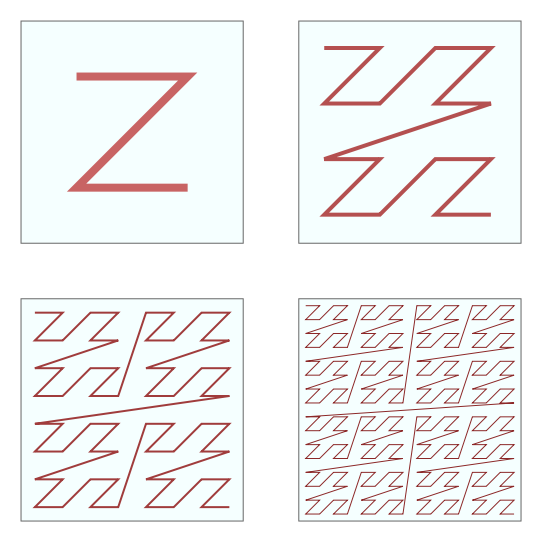
\includegraphics[width=0.8\linewidth]{figures/zcurve.png}
   \caption{4 Iterations of the z-curve in 2D (from wikipedia)}
\end{figure}
In the following it will be explained how the Morton codes can be computed from the center points of the AABBs of out objects.

\subsection{Finding the Root Node AABB}

To calculate the Morton Code for each leaf node AABB, we have to get a representation of the AABB's center points where all coordinates are in range of \mbox{\texttt{[0, 1]}}. Similar to barycentric coordinates, we can use an AABB instead of the usual simplex. This AABB is exactly the AABB of the root node in the BVH. To compute this AABB a simple reduction as covered by Assignment 2 over all leaf node AABBs, that reduces the minimum and maximum value for each axis, is a simple and efficient way to reach this goal.

\subsection{Calculating the Morton code}

At this point all leaf node AABB center points can be represented as 3D point located within the unit cube. To compute an actual single unsigned integral value from them, each coordinate will be scaled to range \mbox{\texttt{[0, 1023]}}, cast into an \texttt{unsigned int} and finally padded with zeroes in between consecutive bits. Figure \ref{fig:swizzle} illustrates this process.
\begin{figure}[!th]
   \centering
   \label{fig:swizzle}
   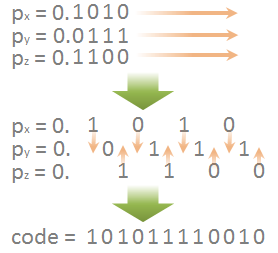
\includegraphics[width=0.8\linewidth]{figures/bitswizzle.png}
   \caption{Scheme for swizzeling the position into a Morton code (from \url{https://devblogs.nvidia.com/parallelforall/thinking-parallel-part-iii-tree-construction-gpu/})}
\end{figure}



\section{Sorting Morton Codes}
\label{sortmortoncodes}

To utilize the Morton codes we have to sort them as well. There are several parallel sort algorithms for GPUs, the one implemented for this assignment is a flavor of radix sort. In this case we will iterate over 32 bit starting from the LSB and calculate prefix sums to reorder the sorting keys (Morton codes) ascending. One iteration for bit at position \texttt{k} can be outlined as:
\begin{enumerate}
  \item Build two arrays of flags A and B, where A is 1 for each key that has it's bit at \texttt{k} set and else 0. B is the inversion of A.
  \item Compute the prefix sums over A and B. Add the maximum value of A to each element in B.
  \item Reorder the keys using A and B as new indices (depending if the key's \texttt{k} bit is set or not).
\end{enumerate}

Sorting the Morton codes this way, is fast using only programming primitives already discussed in Assignment 2. Although there are more efficient algorithms to sort on GPUs, it is deemed that this is sufficient.

\section{Computing Inner Nodes}
\label{computeinnernodes}

As it was already teased in section \nameref{computemortoncodes}, the inner nodes can now be calculated by determining a splitting point in the array of Morton codes. In a naive algorithm this splitting point can be determined starting with the root. This will yield 2 ranges for the two child nodes of the root. The two child nodes now can process their ranges the same way resulting in 2 more split points and all in all 4 ranges of leaf nodes. This process can be continued until all ranges are one element long. This way the constructed BVH is correct, however the GPU utilization is at the very low end. This is because in the first round only one thread is needed to compute the split point and ranges. On a modern GPU with more than 1K possibly parallel executed threads the occupancy is at meagerly 0.001\%. In the next round 2 threads are launched doubling the occupancy as well, but an acceptable occupancy is reached in round 15 with still very low 32\%. However at this point the BVH creation is already completed, given that there are around 30K leaf node objects.

Another approach is to compute the split points of each inner node in parallel. This is possible, because in a binary tree there are exactly \texttt{N-1} inner nodes, if there are \texttt{N} leaf nodes and the split points can be determined without knowing the range before hand. Using those properties we enumerate nodes as shown in figure \ref{fig:nodes}. From here for each node it's range has to be determined. Therefore we have to find out if a node resides on the upper bound or the lower bound of it's range, by comparing neighboring Morton codes. When the direction is set, the other end of the range can be determined with two binary searches, searching for the farthest apart element, but where the length of Morton code's common prefix is only one. If the range is known, the split point is computed using another binary search as one would have implemented it in the naive version. 
\begin{figure}[!th]
   \centering
   \label{fig:nodes}
   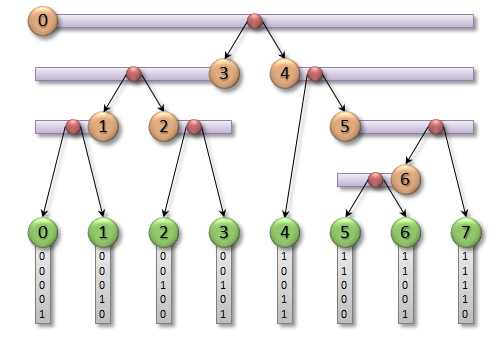
\includegraphics[width=0.8\linewidth]{figures/nodes.png}
   \caption{Enumeration of inner nodes and highlighting their range (from \url{https://devblogs.nvidia.com/parallelforall/thinking-parallel-part-iii-tree-construction-gpu/})}
\end{figure}


Note, that in the parallel approach each thread has to do more work (3 binary searches instead of one) but the benefit is, we can compute every node's split point and range in parallel and do not have to wait for all nodes further up in the hierarchy to finish.

\paragraph{AABBs of Inner Nodes}
Finally the AABBs of each inner node needs to be computed as well. Therefore a slightly modified reduction can be used. Hereby the reduction starts with the leaf nodes, and traverses upwards towards the root. To ensure, that each AABB is correct, atomic flags can be used to ensure that an AABB is computed only once for each inner node and only by the second thread that traverses the tree.

\section{Evaluation}

This is only a rough estimation on how much point each task will be worth:
\begin{itemize}
  \item Computing Morton codes (2P)
  \item Sorting (5P)
  \begin{itemize}
    \item Calculating flags (1P)
    \item Scan (1P)
    \item Reorder (2P)
    \item Reorder other data structures besides the Morton codes e.g. AABBs of leaf nodes (1P)
  \end{itemize}
  \item Inner nodes (4P)
  \item Inner node AABBs (3P)
\end{itemize}

\addtolength{\textheight}{-12cm}   % This command serves to balance the column lengths
                                  % on the last page of the document manually. It shortens
                                  % the textheight of the last page by a suitable amount.
                                  % This command does not take effect until the next page
                                  % so it should come on the page before the last. Make
                                  % sure that you do not shorten the textheight too much.

%%%%%%%%%%%%%%%%%%%%%%%%%%%%%%%%%%%%%%%%%%%%%%%%%%%%%%%%%%%%%%%%%%%%%%%%%%%%%%%%



%%%%%%%%%%%%%%%%%%%%%%%%%%%%%%%%%%%%%%%%%%%%%%%%%%%%%%%%%%%%%%%%%%%%%%%%%%%%%%%%



%%%%%%%%%%%%%%%%%%%%%%%%%%%%%%%%%%%%%%%%%%%%%%%%%%%%%%%%%%%%%%%%%%%%%%%%%%%%%%%%



%%%%%%%%%%%%%%%%%%%%%%%%%%%%%%%%%%%%%%%%%%%%%%%%%%%%%%%%%%%%%%%%%%%%%%%%%%%%%%%%


%\begin{thebibliography}{99}
%
%\bibitem{c1} G. O. Young, ÒSynthetic structure of industrial plastics (Book style with paper title and editor),Ó    in Plastics, 2nd ed. vol. 3, J. Peters, Ed.  New York: McGraw-Hill, 1964, pp. 15Ð64.
%\bibitem{c2} W.-K. Chen, Linear Networks and Systems (Book style).  Belmont, CA: Wadsworth, 1993, pp. 123Ð135.
%\bibitem{c3} H. Poor, An Introduction to Signal Detection and Estimation.   New York: Springer-Verlag, 1985, ch. 4.
%\bibitem{c4} B. Smith, ÒAn approach to graphs of linear forms (Unpublished work style),Ó unpublished.
%\bibitem{c5} E. H. Miller, ÒA note on reflector arrays (Periodical styleÑAccepted for publication),Ó IEEE Trans. Antennas Propagat., to be publised.
%\bibitem{c6} J. Wang, ÒFundamentals of erbium-doped fiber amplifiers arrays (Periodical styleÑSubmitted for publication),Ó IEEE J. Quantum Electron., submitted for publication.
%\bibitem{c7} C. J. Kaufman, Rocky Mountain Research Lab., Boulder, CO, private communication, May 1995.
%\bibitem{c8} Y. Yorozu, M. Hirano, K. Oka, and Y. Tagawa, ÒElectron spectroscopy studies on magneto-optical media and plastic substrate interfaces(Translation Journals style),Ó IEEE Transl. J. Magn.Jpn., vol. 2, Aug. 1987, pp. 740Ð741 [Dig. 9th Annu. Conf. Magnetics Japan, 1982, p. 301].
%\bibitem{c9} M. Young, The Techincal Writers Handbook.  Mill Valley, CA: University Science, 1989.
%\bibitem{c10} J. U. Duncombe, ÒInfrared navigationÑPart I: An assessment of feasibility (Periodical style),Ó IEEE Trans. Electron Devices, vol. ED-11, pp. 34Ð39, Jan. 1959.
%\bibitem{c11} S. Chen, B. Mulgrew, and P. M. Grant, ÒA clustering technique for digital communications channel equalization using radial basis function networks,Ó IEEE Trans. Neural Networks, vol. 4, pp. 570Ð578, July 1993.
%\bibitem{c12} R. W. Lucky, ÒAutomatic equalization for digital communication,Ó Bell Syst. Tech. J., vol. 44, no. 4, pp. 547Ð588, Apr. 1965.
%\bibitem{c13} S. P. Bingulac, ÒOn the compatibility of adaptive controllers (Published Conference Proceedings style),Ó in Proc. 4th Annu. Allerton Conf. Circuits and Systems Theory, New York, 1994, pp. 8Ð16.
%\bibitem{c14} G. R. Faulhaber, ÒDesign of service systems with priority reservation,Ó in Conf. Rec. 1995 IEEE Int. Conf. Communications, pp. 3Ð8.
%\bibitem{c15} W. D. Doyle, ÒMagnetization reversal in films with biaxial anisotropy,Ó in 1987 Proc. INTERMAG Conf., pp. 2.2-1Ð2.2-6.
%\bibitem{c16} G. W. Juette and L. E. Zeffanella, ÒRadio noise currents n short sections on bundle conductors (Presented Conference Paper style),Ó presented at the IEEE Summer power Meeting, Dallas, TX, June 22Ð27, 1990, Paper 90 SM 690-0 PWRS.
%\bibitem{c17} J. G. Kreifeldt, ÒAn analysis of surface-detected EMG as an amplitude-modulated noise,Ó presented at the 1989 Int. Conf. Medicine and Biological Engineering, Chicago, IL.
%\bibitem{c18} J. Williams, ÒNarrow-band analyzer (Thesis or Dissertation style),Ó Ph.D. dissertation, Dept. Elect. Eng., Harvard Univ., Cambridge, MA, 1993. 
%\bibitem{c19} N. Kawasaki, ÒParametric study of thermal and chemical nonequilibrium nozzle flow,Ó M.S. thesis, Dept. Electron. Eng., Osaka Univ., Osaka, Japan, 1993.
%\bibitem{c20} J. P. Wilkinson, ÒNonlinear resonant circuit devices (Patent style),Ó U.S. Patent 3 624 12, July 16, 1990. 
%
%
%
%
%
%
%\end{thebibliography}




\end{document}
